\PassOptionsToPackage{table}{xcolor}
\documentclass[11pt]{article}
%
%%%%%%%%%%%%%%%%%%%%%%%%%%%%%%%%%%%%
%% Common preamble
%%%%%%%%%%%%%%%%%%%%%%%%%%%%%%%%%%%%
% PAGE
\newcommand{\tuta}{\emph{T.~absoluta}}
\newcommand{\infest}{\rho}
\newcommand{\totinf}{\rho_{\mathrm{T}}}
\newcommand{\suitable}{\epsilon}
%% \usepackage{fullpage} % uncomment this when changing to jour/conf style
% FONTS
\usepackage{textcomp}
\usepackage{lmodern} % enhanced version of computer modern
\usepackage[T1]{fontenc} % for hyphenated characters and textsc in section title
\usepackage{xr}
\externaldocument[S:]{mcnitt_tuta_supplementary}
\usepackage{microtype} % some compression
\usepackage{times}
\usepackage{setspace} % For double line spacing
\doublespacing
\usepackage[left=1in,top=1in,right=1in,bottom=1in]{geometry}
\usepackage[pagewise]{lineno}
\linenumbers
\usepackage{marvosym}
%% \newcommand\wordcount{\immediate\write18{texcount -sub=section \jobname.tex  | grep ``Section'' | sed -e 's/+.*//' | sed -n \thesection p > 'count.txt'} (\input{count.txt}words)}
% MATH
\usepackage{amssymb}
\usepackage{mathtools} % contains amsmath which comes with align
\usepackage{amsthm} % newtheorem stuff
\usepackage{bm} % for bold math (use $\boldsymbol{}$)
% COLOR
\usepackage[usenames,dvipsnames]{color}
%%
% REFERENCING
% JM: Below is for affiliations
\usepackage{authblk}
% BIBLIOGRAPHY
\usepackage[square,sort&compress,numbers]{natbib} %sorts bibs when they are collectively cited
\usepackage[colorlinks=true,pdfborder={0 0 0},citecolor=RoyalBlue,linkcolor=black,urlcolor=Magenta]{hyperref}
\usepackage{cleveref} %%% IMPORTANT: cleveref comes before \newtheorem commands
   \crefname{figure}{Figure}{Figures}
   \crefname{table}{Table}{Tables}
   \crefname{theorem}{Theorem}{Theorems}
   \crefname{lemma}{Lemma}{Lemmas}
   \crefname{claim}{Claim}{Claims}
   \crefname{section}{Section}{Sections}
   \crefname{observation}{Observation}{Observations}
   \crefname{note}{Note}{Notes}
%%
% TABLES
\usepackage{multirow}
%% \usepackage{ctable} % provides toprule, bottomrule, midrule
\usepackage{array} % new implementation of tabular & array with lots of enhancements
%%
% FIGURES
\usepackage{graphicx}
\graphicspath{./figs}
\usepackage{grffile} % to set right names of files
%%
% CAPTIONS
\usepackage{caption}
\usepackage{subcaption} % supersedes subfigure & subfloat. try using options
%%
% LISTS
\usepackage{enumitem} %\begin{itemize}[leftmargin=*]
%% inline
\newlist{inline}{enumerate*}{1}
\setlist[inline]{before=\unskip{: }, itemjoin={{; }}, itemjoin*={{; and }}, label={(\roman*)}}
\usepackage{silence}
\WarningFilter{ctable}{Transparency disabled:}
\WarningFilter{xcolor}{Incompatible color}
% ALGO
\usepackage[ruled,linesnumbered]{algorithm2e}
%% comments & todo
\newcommand{\reportingCells}{\mathcal{C}_R}
\newcommand{\similarity}{\mathcal{S}}
\newcommand{\aacomment}[1]{({\color{magenta}AA: #1})}
\newcommand{\mmcomment}[1]{({\color{green}MM: #1})}
\newcommand{\tbcomment}[1]{({\color{blue}TB: #1})}
\newcommand{\mrccomment}[1]{({\color{red}MRC: #1})}
\newcommand{\jmcomment}[1]{({\color{cyan}JM: #1})}
\usepackage[colorinlistoftodos]{todonotes}
\newcommand{\TODO}[1]{\todo[inline,color=red!10,size=\small]{#1}}
%% COMMANDS
\newcommand{\comp}[1]{\overline{#1}}  %{\widetilde{#1}}
\DeclareMathOperator{\Var}{Var}
\DeclareMathOperator{\Cov}{Cov}
\DeclareMathOperator{\bigo}{O}
\DeclareMathOperator{\bigom}{\Omega}
\DeclareMathOperator{\davg}{d_{avg}}
\DeclareMathOperator*{\argmax}{arg\,max}
\DeclareMathOperator*{\argmim}{arg\,min}
% Note: \deg is already defined
\newcommand{\expect}{\mathbb{E}}
%
\newcommand{\ceil}[1]{\left\lceil #1 \right\rceil}
\newcommand{\floor}[1]{\left\lfloor #1 \right\rfloor}
%
\newcommand{\reals}{\mathbb{R}}
\newcommand{\field}{\mathbb{F}}
\newcommand{\integers}{\mathbb{Z}}
\newcommand{\pshort}{p_s}
\newcommand{\plocal}{p_{\ell}}
\newcommand{\pld}{p_{\ell d}}
\newcommand{\asd}{\alpha_s}
\newcommand{\afm}{\alpha_{\ell}}
\newcommand{\ald}{\alpha_{\ell d}}
\newcommand{\produce}{\mathrm{Prod}}
\newcommand{\veg}{\mathrm{V}}
\newcommand{\temp}{\mathrm{T}}
\newcommand{\consume}{\mathrm{Pop}}
\newcommand{\locality}{{L}}
\newcommand{\export}{\mathrm{Export}}
\newcommand{\import}{\mathrm{Import}}
\newcommand{\process}{\mathrm{Proc}}
\newcommand{\moore}{\mathrm{M}}
\newcommand{\mooreRange}{r_\mathrm{M}}
%
\newtheorem{theorem}{Theorem}[]{\bfseries}{\itshape} 
\newtheorem{lemma}[theorem]{Lemma}{\bfseries}{\itshape}
\newtheorem{claim}[theorem]{Claim}{\bfseries}{\itshape}
\theoremstyle{definition}
\newtheorem{definition}[theorem]{Definition} % {\bfseries}{\itshape}
\newtheorem{observation}[theorem]{Observation} % {\bfseries}
\newtheorem{condition}[theorem]{Condition} % {\bfseries}{\itshape}
\newtheorem{note}[theorem]{Note} % {\bfseries}{\itshape}
% ROMAN NUMERALS
\makeatletter
\newcommand{\rmnum}[1]{\romannumeral #1}
\newcommand{\Rmnum}[1]{\expandafter\@slowromancap\romannumeral #1@}
\makeatother
%%
% TWO VERSIONS
%% \usepackage{etoolbox}
%% \newtoggle{withappendix}
%% \toggletrue{withappendix} % comment this if you want journal version
%% Usage: iftoggle{withappendix}{}{}
%%
%% math operator
%% \DeclareMathOperator{\sgn}{sgn}
% CODEBOX
%% \usepackage[framemethod=tikz]{mdframed}
%% \newmdenv[linecolor=black!10,innerlinewidth=0pt, roundcorner=4pt,innerleftmargin=6pt,
%% font=\ttfamily,innerrightmargin=6pt,innertopmargin=6pt,
%% innerbottommargin=6pt,backgroundcolor=black!10]{codeblock}
%%%%%%%%%%%%%%%%%%%%%%%%%%%%%%%%%%%%
%% preamble ends
%% from now on, draft specific
%%%%%%%%%%%%%%%%%%%%%%%%%%%%%%%%%%%%
%% \RequirePackage[l2tabu, orthodox]{nag}
\makeatletter
\renewcommand\AB@affilsepx{, \protect\Affilfont}
\makeatother
% Title on edge of suggested length
\title{Assessing the Multi-pathway Threat from an Invasive Agricultural
Pest: \emph{Tuta~absoluta} in Asia}
%% \title{A Multi-pathway Model to Assess the Threat of Invasive Agricultural
%% Pests: Case Study of \emph{Tuta~absoluta} in Asia}
\author[1]{Joseph~McNitt}
\author[2]{Young~Yun~Chungbaek}
\author[2]{Henning~Mortveit}
\author[2]{Madhav~Marathe}
\author[3]{Mateus~R~Campos} %%ibeiro~de
\author[3]{Nicolas~Desneux}
\author[4,5,6]{Thierry~Br\'{e}vault}
\author[7]{Rangaswamy Muniappan}
\author[2]{Abhijin~Adiga}
\affil[1]{Epic Systems Corporation, United States}
\affil[2]{Biocomplexity Institute \& Initiative, University of Virginia}
\affil[3]{French National Institute for Agricultural Research}
\affil[4]{BIOPASS, CIRAD-IRD-ISRA-UCAD, Dakar, Senegal}
\affil[5]{CIRAD, UPR AIDA, F-34398 Montpellier, France}
\affil[6]{Universit\'{e} de Montpellier, CIRAD, Montpellier, France}
\affil[7]{Feed the Future Integrated Pest Management Innovation Lab,
Virginia Tech}
\date{}
\setcounter{Maxaffil}{0}
\renewcommand\Affilfont{\itshape\small}

\begin{document}
\maketitle

\begin{abstract}
Modern food systems facilitate rapid dispersal of pests and pathogens
through multiple pathways. The complexity of spread dynamics and data
inadequacy make it challenging to model the phenomenon and also to prepare
for emerging invasions. We present a generic framework to study the
spatiotemporal spread of invasive species as a multi-scale propagation
process over a time-varying network accounting for climate, biology,
seasonal production, trade, and demographic information. Machine learning
techniques are used in a novel manner to capture model variability and
analyse parameter sensitivity. We applied the framework to understand the spread
of a devastating pest of tomato, \emph{Tuta absoluta}, in South and
Southeast Asia, a region at the frontier of its current range. Analysis
with respect to historical invasion records suggests that even with modest
self-mediated spread capabilities, the pest can quickly expand its range
through domestic city-to-city vegetable trade. Our models forecast that
within five to seven years, \tuta{} will invade all major vegetable growing
areas of Mainland Southeast Asia assuming unmitigated spread. Further, we
show that monitoring high consumption areas, and targetted interventions
in major production regions can help in early detection and reducing the
speed of spread.
\end{abstract}
%%
\section{Introduction}
As the intensity of trade and human mobility increase, so does the rate of
exotic species invasions~\cite{hulme2009trade}. Climate change and the
detrimental impact of intensive agriculture on natural resources further
aggravate this problem~\cite{early2016global}.  Understanding the dynamics
of invasive species spread is imperative for achieving zero hunger, no
poverty, good health and well being, which are among the sustainable
development goals drafted by the United
Nations~\cite{un_sustainable_development}. Models play an important role in
predicting the spatiotemporal spread, identifying roles of different
pathways, assessing efficacy of control strategies, and exposing gaps in the
understanding of the
phenomenon~\cite{cunniffe2015thirteen,epstein2008model}. However, impending
invasions of agricultural pests present difficult challenges.  Accounting
for multiple drivers of dispersal invariably makes the model complex.  At
the same time, data inadequacy makes it nearly impossible to calibrate and
validate these models. Despite these limitations, a natural goal for a
modeller is to provide useful insights into the mechanisms of spread, and
thus help design effective policies for its prevention and mitigation.

Network propagation models have been widely used to study large interacting
biological, social and technical systems. Some examples include infectious
disease spread, online social networks, cascading failures in
infrastructure networks~\cite{barrat2008dynamical}.  Increasingly,
they are being applied to study invasive species
dynamics~\cite{douma2016pathway,carrasco2010unveiling,nopsa2015ecological}.
Unlike pest risk maps generated by species distribution
models~\cite{pearson2007species}, the resulting dynamics of such a
validated model yields a causal description of the underlying complex
system. Here, we present a multi-pathway propagation model to study the
spread of invasive agricultural pests. The model accounts for both
self-mediated and human-mediated spread and effectively encapsulate the spatial
heterogeneity, temporal variations and multi-scale nature of the
propagation mechanisms.

We applied this framework to study the spread of the South American tomato
leafminer or \emph{Tuta absoluta}, a pest of the tomato crop and
representative of recent biological invasions that have significantly
perturbed global food production.  Indigenous to South America, \tuta{} was
accidentally introduced to Spain in~2006, and since then has rapidly
spread throughout Europe, Africa, Western and Central Asia, the Indian
subcontinent, and parts of Central
America~\cite{desneux2010biological,biondi2017}. With tomato being a
commercially important crop, this invasion has had significant global
impact~\cite{campos2017western}. It is well accepted that trade
played a critical role in \tuta{}'s rapid spread. On multiple occasions it
has been discovered in packaging stations and its spread pattern is
correlated with prime trade routes~\cite{karadjova2013tuta}. Our study
region is South and Southeast Asia-- a region at the frontier of its
current range -- comprising of 10 countries: members of the Association of
Southeast Asian Nations (ASEAN) and Bangladesh.  In recent years, there
has been a thrust to improve vegetable production in all the countries of
this region. With the pest having already spread to major
tomato producing areas in Bangladesh, there is a
high chance that it will be introduced to the remaining countries in the
near future. Such invasions can have devastating effect on the economy and
livelihood of farmers.  Moreover, the invasion in Mainland Southeast Asia in
particular is a serious threat to China, the largest producer of tomato,
and Australasian neighbours. To our knowledge, this is the first study that
explicitly considers multiple pathways of introduction and spread of
\tuta{}.  Earlier modelling efforts have only accounted for ecological
aspects and self-mediated
spread~\cite{desneux2010biological,tonnang2015identification,guimapi2016modeling}.

Our contributions are multifold. We provide a generic data-driven approach
to build complex multi-pathway models. We identified, analysed, and fused
disparate datasets corresponding to climate (temperature, precipitation,
elevation), biology (host preference, suitability, population growth),
production, and agricultural commodity flow (domestic trade, imports,
exports, vegetable processing, human population). We estimated the
spatiotemporal distribution of host crops by integrating information from
research articles, annual reports, and models. Trade flows were estimated
using a gravity model approach.  Machine learning techniques such as
clustering and decision-tree algorithms were used for parameterization, to
capture model variability and study parameter sensitivity resulting from
inadequate incidence reports and understanding of the pest dynamics.

From an application perspective, the analysis provides valuable insights
into the dynamics of \tuta{} spread.  Our analysis with respect to
historical invasion records indicates two possible explanations for the
spread of \tuta{} in Bangladesh, one with trade as the dominant pathway and
the other without. The former explanation suggests that even with slow
self-mediated dispersal, the pest could have rapidly expanded its range
aided by domestic tomato trade. Under the assumption that trade is an
important pathway, country specific analysis shows that once introduced to
a major production area, the pest will spread all over the country within
two to three years. Since densely populated urban centres attract trade
inflows, high production regions close to such areas are particularly
vulnerable to attacks. We also show that quarantining a few key production
areas can contain the spread.

%%
\section{Methods}
%%
\paragraph{Data.} The global datasets used in the model and for analysis
are described in Table~\ref{S:tab:data} of the supplement. Country specific
data on seasonal production, consumption, processing, and trade was obtained
from websites of agriculture ministries, research articles and technical
reports (Table~\ref{S:tab:countryData} in the supplement). Almost all the
datasets used are openly available. Some information was provided by local
contacts in Bangladesh (for e.g., \tuta{} incidence reports in
Table~\ref{S:tab:bgdData}), Vietnam, and Cambodia.
%%
\paragraph{\tuta{} biology.}
The tomato leafminer exhibits a short life cycle of about 24--38 days
(temperature at $25\pm3^\circ$C), from egg to adult, as it is a
multivoltine species with overlapping generations in the
field. It causes serious damage to
numerous solanaceous crops such as eggplants, potatoes, and especially
tomato crops~\cite{sylla2018}. It penetrates into tomato leaves, stems, or
fruits, wherein it feeds and develops by creating conspicuous mines as well
as galleries. Considering the warm weather throughout the year,
particularly in the dry season, the study region presents ideal conditions
for rapid development and spread of \tuta{}. Pest risk
analysis~\cite{tonnang2015identification} shows that the Ecoclimatic Index
for this region is above~$50$ (highly suitable). Spatial distribution
assessment survey of \tuta{} eggs has shown its high dispersive capacity in
tomato producing areas~\cite{martins2018assessing}. The dispersion in a
tomato cultivation starts mainly at the periphery and
the pest is able to migrate between tomato farms to generate egg aggregation at the
crop boundaries. The pest spread behaviour among seasonal crop resources
is often non-random and directional~\cite{martins2018assessing}.
Sylla~et~al.~\cite{sylla2018} analysed host preference of~\tuta{} in France
and Senegal. While the highest preference is for tomato, it can survive
well on eggplant and potato, which happen to be major vegetable crops in
the study region. However, since \tuta{} primarily attacks leaves of
eggplant and potato, the chance of the pest spreading through trade of
these crops seems to be low.
%%~\cite{guedes2012tomato}
%%
\paragraph{Multi-pathway spread model.} We developed a stochastic
multi-scale propagation model to simulate the multi-pathway spread
of~\tuta{}. Key concepts are illustrated in Figure~\ref{fig:concept}. The
study region is divided into cells -- the smallest spatial units -- by overlaying a grid
(0.25\textdegree~$\times$~0.25\textdegree). Each cell is in one of the
three states: susceptible ($S$) denoting pest free state, exposed ($E$)
denoting that the pest has been introduced but the population has not yet
built up to influence other cells, and infectious ($I$) denoting that the
pest has established and the cell can influence its neighbours. The cell
states are updated in discrete time steps, where the interval between
successive time steps corresponds
to a month.  The probability that a cell~$v$ transitions from state~$S$
to~$E$ is determined by (i)~suitability of the cell for \tuta{} to
establish at that time step~$\suitable(v,t)$ and (ii)~influence of
``neighbouring'' cells in state~$I$ depending on the pathway. An exposed
cell transitions to state~$I$ after a latency period of~$\ell$ time steps.
This is the time required for the population to build up to infect other
cells.  Once the pest has established in a cell, the cell remains infected
forever, a fair assumption considering that, historically, eradication of
\tuta{} has not been successful\footnote{The only exception is United
Kingdom where the pest was detected early and
eradicated.}.  The
infectiousness of a cell~$\infest(v,t)$ is modelled as a linear function of
host presence at time~$t$, for which we use the weighted sum of production
volume of tomato, eggplant, and potato in that cell at time~$t$. The
weights correspond to relative carrying capacity of \tuta{} on the three
hosts~\cite{sylla2018}.
%%~(\url{https://gd.eppo.int/reporting/article-340})
%%
\begin{figure}[t]
\centering
\begin{subfigure}[b]{.4\textwidth}
    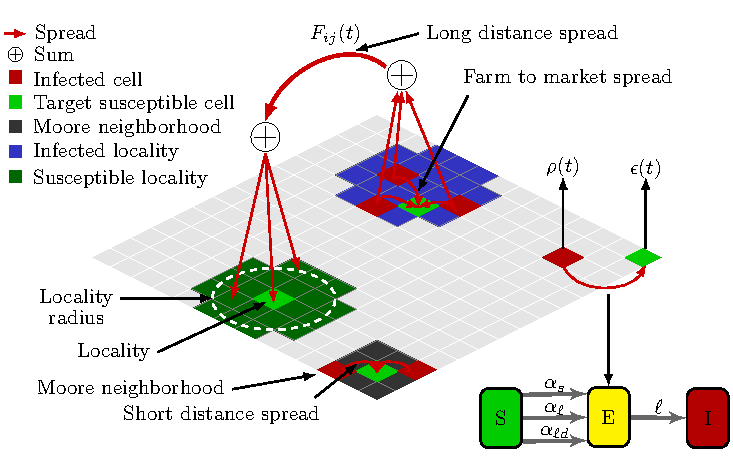
\includegraphics[width=1.1\textwidth]{figs/model_schematic.pdf}
\caption{\label{fig:concept}}
\end{subfigure}
%%
\begin{subfigure}[b]{.56\textwidth}
    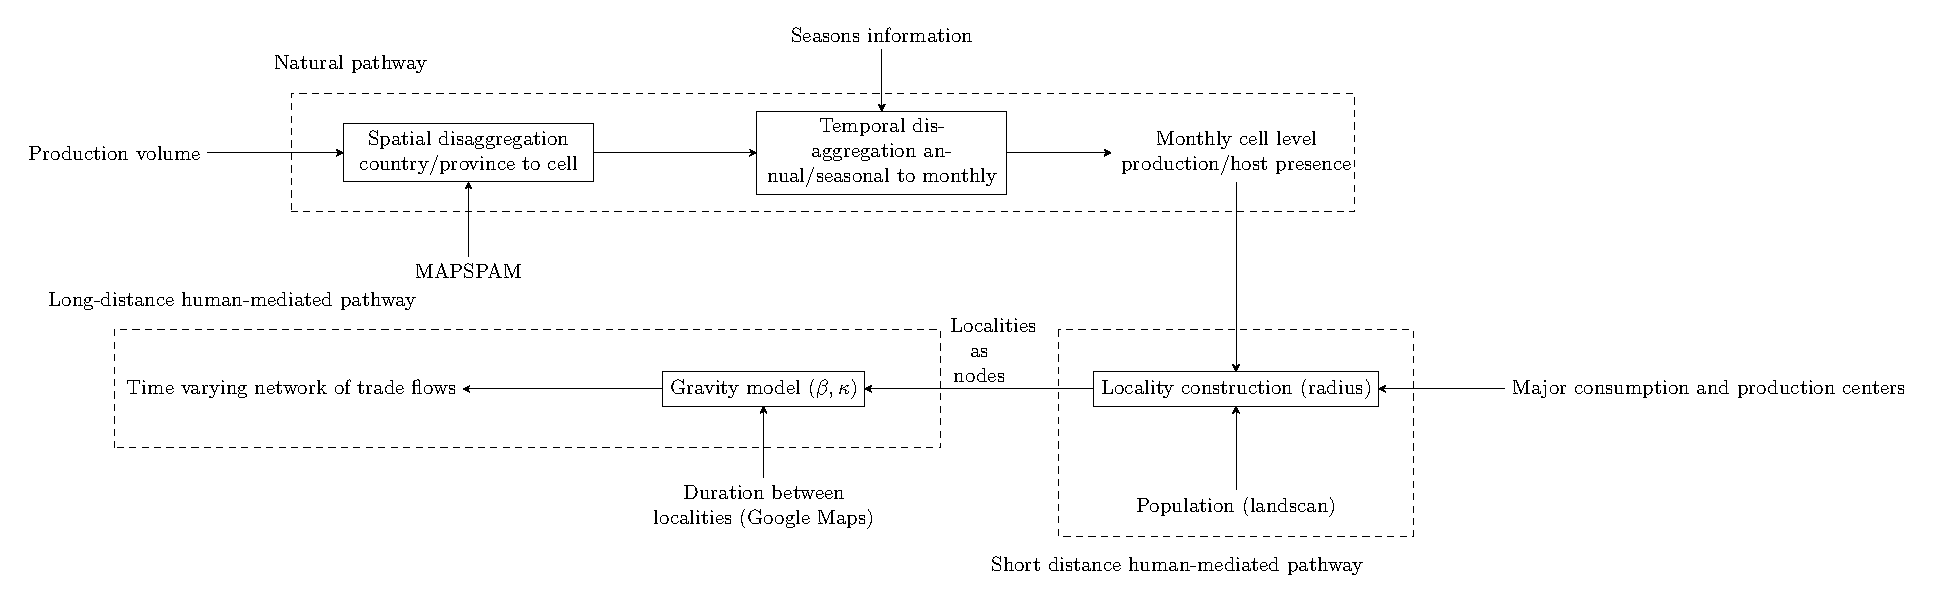
\includegraphics[width=1.05\textwidth]{figs/pipeline.pdf}
\caption{\label{fig:pipeline}}
\end{subfigure}
\caption{\textbf{The multi-pathway model.} (a)~The network structure,
pathways and dynamics are captured in the illustration.
%% , which is
%% approximately~$27.8\mathrm{km}\times\mathrm{27.8km}$ at the equator. 
%% These
%% dimensions are comparable to that used in the cellular automata model of
%% Guimapi~et.~al.~\cite{guimapi2016modeling} ($25\mathrm{km}\times25\mathrm{km}$). Details of locality construction are in Section~\ref{S:sec:locality}. 
%% Long distance human-mediated dispersal is modeled
%%las the spread between localities through. 
Also shown are the states and factors
that influence state transitions: infectiousness of a neighbouring cell, suitability
of the cell for pest establishment, pathway parameters and latency period.
\label{fig:modelConcept}
(b)~\textbf{Pipeline.} The process of constructing the spatiotemporal
network of cells is outlined. Key modules are highlighted along with 
input data.}
\end{figure}
%%

There are three pathways by which a cell can become infected:
short-distance dispersal, local human-mediated dispersal and long-distance
dispersal. Short-distance dispersal captures the spread through natural
means; from an infested cell to cells in its Moore neighbourhood of
range~$\mooreRange$.  The probability that a susceptible cell gets exposed
(E) at time step~$t$ through short-distance spread is as follows:
%%
\begin{linenomath}
\begin{align}\label{eqn:pshort}
    \pshort(v,t)=\suitable(v,t)\bigg(1-
    \exp\Big(-\asd\sum_{v'\in\moore_v(\mooreRange)}\infest(v',t)\Big)\bigg)\,.
\end{align}
\end{linenomath}
%%
The probability depends on the suitability of the cell~$\suitable(v,t)$,
infestation level of each neighbouring cell in the Moore neighbourhood with
range~$\mooreRange$,~$\infest(v',t)$, and the scaling factor,~$\asd$, which
is the transmission rate for this pathway. The function form is explained
in Section~\ref{S:trans}.

For human-assisted spread we identified large urban areas in the region
which we refer to as {\it localities} (Figure~\ref{fig:modelConcept}) and
considered interactions within and between localities. These areas have
high trade flows due to consumption or production and house the necessary
infrastructure: wholesale markets, traders, and distributors.  Each
\emph{locality} consists of all grid cells which are within a certain
distance (determined by \emph{locality radius}) from its corresponding
centre. Local human-mediated dispersal is modelled as the spread between
cells belonging to a locality.  Every cell~$v$ is influenced by cells in
its locality~$\locality$ based on their infectiousness.  The expression is
similar to that in equation~\eqref{eqn:pshort}, but with cells in the locality
instead of the Moore neighbourhood
%%
\begin{linenomath}
\begin{align}\label{eqn:plocal}
    \plocal(v,t)=\suitable(v,t)\bigg(1-
    \exp\Big(-\afm\sum_{v'\in\locality}\infest(v',t)\Big)\bigg),
\end{align}
\end{linenomath}
%%
where~$\afm$ is the scaling factor. The details of locality construction
are provided in Section~\ref{S:sec:locality} of the supplement.

Long-distance human-mediated dispersal corresponds to spread through trade
between localities. For this purpose, we considered only tomato trade as
there is not much evidence of \tuta{} spreading through trade of other
hosts. We modelled domestic trade using a gravity model approach accounting
for tomato production, processing, imports, and exports in each locality,
and the travel time between localities.  The probability of spread is
directly proportional to the trade flow~$F_{ij}$ from one locality ($i$) to
another ($j$).  Suppose cell~$v$ belongs to locality~$i$. Then, the
probability of cell~$v$ transitioning from~$S$ to~$E$ due to long-distance
human-mediated dispersal is given by:
%%
\begin{linenomath}
\begin{align}\label{eqn:pld}
    \pld(v,t)=\suitable(v,t)\bigg(1-
    \exp\Big(-\ald\sum_{j\ne i}\sum_{v'\in\locality(j)}F_{ji}\infest(v',t)\Big)\bigg),
\end{align}
\end{linenomath}
%%
where~$\ald$ is the pathway scaling factor.  The model parameters and their
values are summarised in Table~\ref{tab:param}.
%%
\begin{table}[t]
\caption{Model parameters, their values and notes on parameter choices and
ranges.\label{tab:param}}
    \centering
	\small
\rowcolors{2}{white}{gray!15} % For this to work, put \PassOptionsToPackage{table}{xcolor} before \documentclass
    \begin{tabular}{p{.07\textwidth}p{.39\textwidth}p{.47\textwidth}}
    %{cp{.25\textwidth}p{.25\textwidth}lr}
		\hline		
		Parameter & Description & Value/range \\
\hline		
\hline
$\mooreRange$ & Range of Moore neighbourhood & $\{1,2,3\}$ corresponding to
spread per month of 
approximately~$25$km,~$50$km and~$75$km
respectively~\cite{guimapi2016modeling,martins2018assessing}. \\
%% $\suitable$ & Suitability threshold \\
$\ell$ & Latency period to transition from $E$ to $I$ & $\{1,2,3\}$ months
based on the time for the pest to complete life cycle (\tuta{} biology in
Methods). \\
season & Disaggregation of annual production to monthly values
& \emph{Uniform} throughout the year or \emph{seasonal} based on regression
analysis (Methods). \\
$\beta$ & Gravity model distance function exponent & $\{0,1,2\}$ \\
$\kappa$ & Gravity model distance function cut-off & Between $4$ to $16$ hours
of travel time. \\
seed & Location and time of initial infestation & Scenarios based on
countries (see Table~\ref{S:tab:seeds})\\
locality radius & Determines cells assigned to a locality & 100km (See
Section~\ref{S:sec:locality} in the supplement for locality construction
and analysis) \\\hline
$t_s$ & Time of initial infestation during parameterization & $\{3,4,5\}$ corresponding
to March, April and May respectively based on first report in
Bangladesh~\cite{hossain2016first}. \\
%% $\infest$ & Infectivity of a cell based on amount of production & \\
$\asd$ & Short-distance spread scaling factor & In the interval $[0,500]$.\\
$\afm$ & Local human-mediated dispersal scaling factor & In the interval $[0,500]$.\\
$\ald$ & Long distance spread scaling factor & In the interval $[0,500]$.\\
\hline
\end{tabular}
\end{table}
%%
\paragraph{Network construction.} 
Figure~\ref{fig:pipeline} provides a schematic of the network construction.
The first step was to estimate monthly production volume of tomato,
eggplant, and potato for each cell. We estimated annual production in each
cell followed by disaggregation to monthly production. The annual
production was estimated using the vegetable production available at the
highest resolution for each country (at the level of province to just one
value for the entire country) and a synthetic dataset called Spatial
Production Allocation Model~\cite{spam}. For monthly production, we
used linear regression to model the production rate as a function of
precipitation, temperature, and elevation. Seasonal tomato and eggplant
production data for different regions of Philippines was used. For most of
the other countries only qualitative information on seasonal production
is available (Table~\ref{S:tab:countryData}). The regression function was
applied to locations of these countries where this information is
available and visually compared available data. The details are in
Section~\ref{S:sec:prod} of the supplement.

To model locality-to-locality trade, we applied the approach of
Venkatramanan~et~al.~\cite{venkatramanan2019modeling}
with some modifications. We modelled the flow of fresh tomato crop between
markets based on the following assumptions: (i)~the total outflow from a
city depends on the amount of produce in its surrounding regions and
imports from countries outside the focus region at time~$t$, and (ii)~the
total inflow depends on total consumption, processing demand, and exports
from the city to countries outside the focus region. The details are in
Section~\ref{S:sec:netcon}.  Trade between countries of the focus region
was not modelled as there is no adequate information on ports of entry or
monthly flow volumes.

\paragraph{Parameterization and experiment design.}
The goodness of fit of a parameter instance was determined by comparing the
simulation output with \tuta{} incidence reports
(Figure~\ref{fig:bgdClassA} and Table~\ref{S:tab:bgdData} for Bangladesh). The
spread was simulated with infestation starting from the location of first
report. For each cell, empirical probability that
it is in state~$I$ at time~$t$ was computed (averaged over 100
repetitions). The output was compared to ground truth using a similarity
function adapted from~\cite{carrasco2010unveiling}.  Let~$v$ be a reporting
cell and~$t_v$ denote the month of the actual report of pest presence.  To
account for uncertainty in reporting, we consider a time
window~$U_\tau=[t_v-\tau,t_v+\tau]$ during comparison, where~$\tau$ is the
uncertainty parameter. We set~$\tau=2$, that is, error within $\pm2$ months is
tolerated.  Supposing~$\reportingCells$ is the set of cells corresponding
to ground truth,  and ~$p(C,v,t)$ is the empirical probability that cell~$v$
is infected at time~$t$ for the input configuration~$C$, then the similarity~$\similarity$ is
given by
%%
\begin{linenomath}
\begin{align}\label{eqn:similarity}
    \similarity(C)=\frac{1}{|\reportingCells|}\sum_{v\in\reportingCells} \Big(\sum_{t\in U_\tau}p(C,v,t)
    + \sum_{t\notin U_\tau}\big(1-p(C,v,t)\big) \Big)\,.
\end{align}
\end{linenomath}
%%
Note that $\similarity(C)$ attains a maximum value of one when the simulation output is a
perfect match (within the error tolerance limit). Parameter space
exploration was conducted in multiple iterations (the ranges or values of
model parameters are in Table~\ref{tab:param}). First, we coarsely sampled
the space. Then, with model parameters as independent variables and the goodness
of fit measure defined in~\eqref{eqn:similarity} as the dependent variable,
we used a Classification and Regression Trees (CART) approach to identify
subspaces for which the similarity score was high and rejected subspaces for
which it was low. Based on this, in the subsequent phases, we
refined our search to improve the parameterization. Simulations were
performed for more than~$500,000$ parameter combinations using a high
performance computing cluster. Configurations with similarity score
$\similarity(C)\ge0.75$ were chosen for further analysis.

\paragraph{Analysis of spread pattern.} The objective here is to analyse
the variability in the simulation outcomes within the set of best fit
configurations. We leverage well-known machine learning techniques in a
novel way to address this question. The methodology is 
outlined in Figure~\ref{fig:clusterOutline}. First, we cluster
the simulation outputs (time and cell indexed empirical probabilities) of
selected configurations from the parameterization phase. This step captures
the variability in outcomes; simulation outputs belonging to different
clusters can be considered to be significantly different from one another.
In the second step, we attempt to infer relationships between model
parameters and cluster membership. To this end, our approach is to cast this as a
classification problem using CART with model parameters as the features
and cluster index as the label. The relationships
are inferred from the decision tree that resulted from the algorithm.
To avoid any bias introduced by the clustering algorithm, we also apply more
than one method -- hierarchical agglomerative clustering and
the $k$-means algorithm. In both cases, we use the Euclidean
distance as the distance measure to compare two simulation outputs. The
analysis is repeated for different values of~$k$, the number of clusters.
More details are provided in Section~\ref{S:sec:cluster} of the supplement.
%%
\begin{figure}[htb]
    \centering
    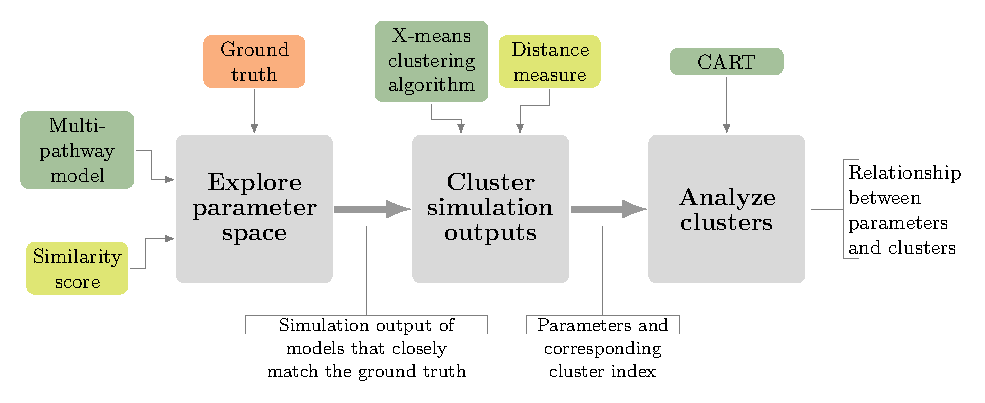
\includegraphics[width=.8\textwidth]{figs/spread_analysis.pdf}
    \caption{Outline of the process used for analysing the multi-pathway spread. \label{fig:clusterOutline}}
\end{figure}
%%
\section{Results}
\paragraph{Variability in spread pattern.} The clustering analysis of the
configurations selected during the parameterization phase (approximately
8000 of them) reveals two distinct spread patterns primarily determined by
the pathway parameters.  The first class of models
(Figure~\ref{fig:bgdClassA}), referred to as Class~A, is characterised by
the absence of long-distance human-mediated spread ($\ald$ negligible) and
brisk spread between geographically adjacent cells, driven by the latency
period~$\ell$, the Moore range~$\mooreRange$, and the short-distance scaling
factor~$\asd$. In contrast, for Class~B models
(Figure~\ref{fig:bgdClassB1}), the long-distance pathway~($\ald$) plays a
significant role  and there is relatively slow spread between
geographically adjacent neighbours. Both hierarchical clustering and
$k$-means clustering (Figures~\ref{S:fig:cartAgglomerative}(b)
and~\ref{S:fig:cartkmeans}(a)) are consistent in this regard.

%%
\begin{figure}[t]
    \centering
\begin{subfigure}[b]{.3\textwidth}
    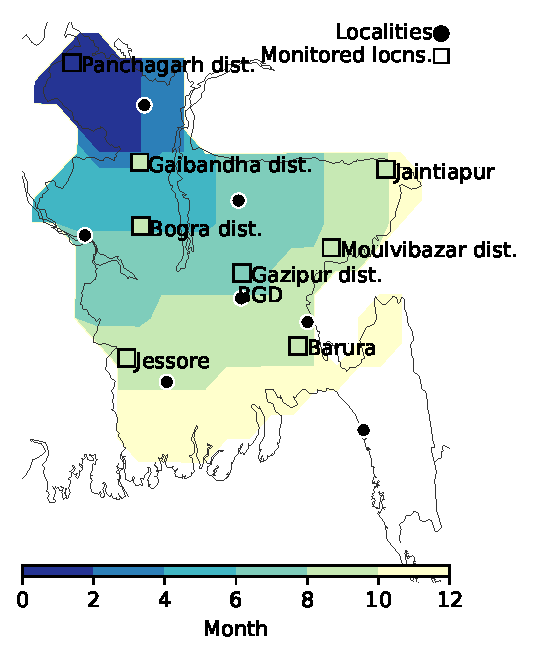
\includegraphics[width=\textwidth]{../cellular_automata/results/contour/BGD_model-A.pdf}
    \caption{Class~A \label{fig:bgdClassA}}  %%($\ald=0$)
\end{subfigure}\hspace{.5cm}
\begin{subfigure}[b]{.3\textwidth}
    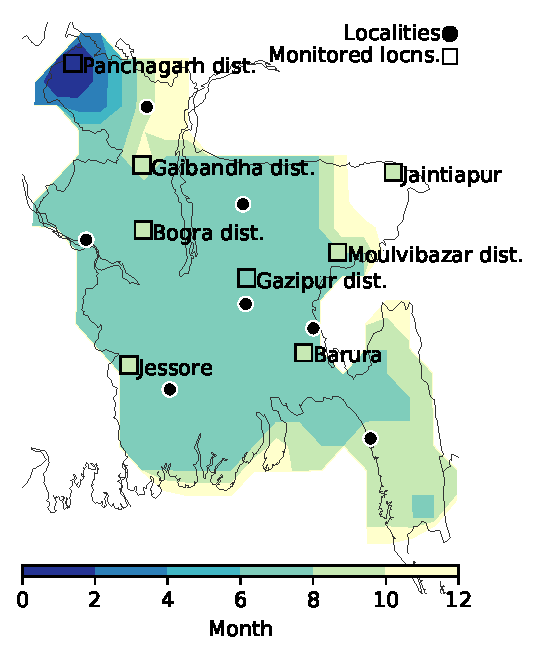
\includegraphics[width=\textwidth]{../cellular_automata/results/contour/BGD_model-B_m1_l3.pdf}
    \caption{Class~B \label{fig:bgdClassB1}} %%($\ald>0$)
\end{subfigure}
\begin{subfigure}[b]{.32\textwidth}
    \centering
    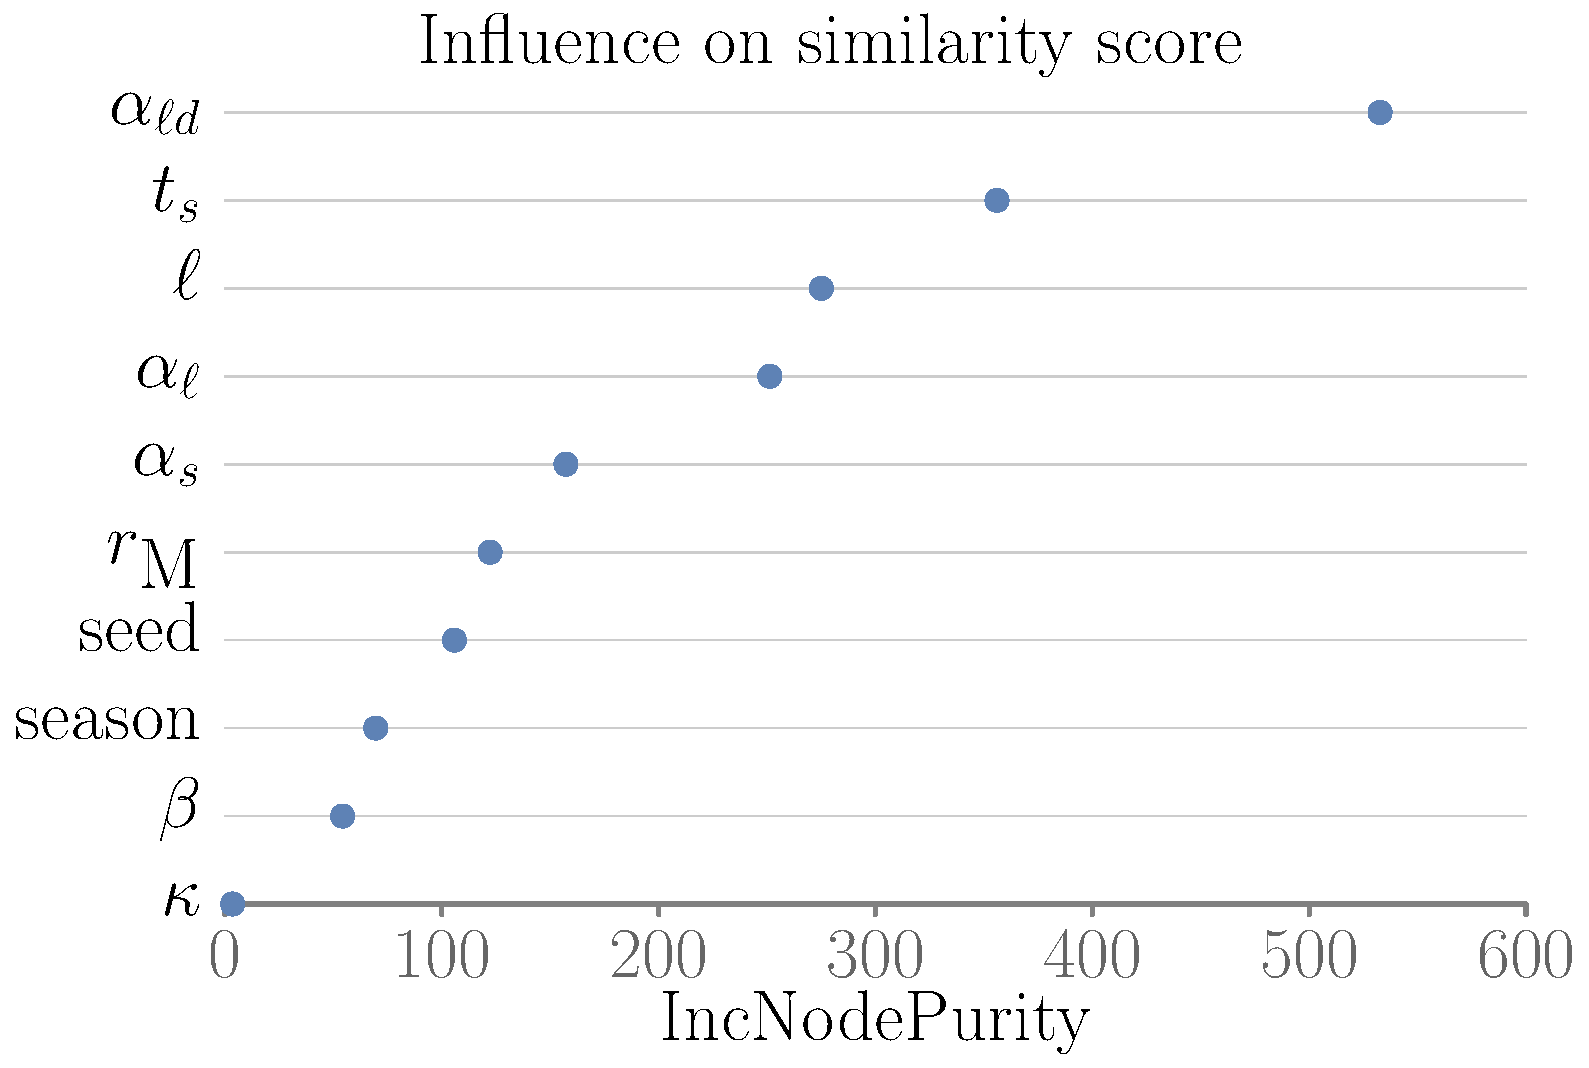
\includegraphics[width=0.9\textwidth]{../cellular_automata/results/rf/rf_importance_all_mdi.pdf}
    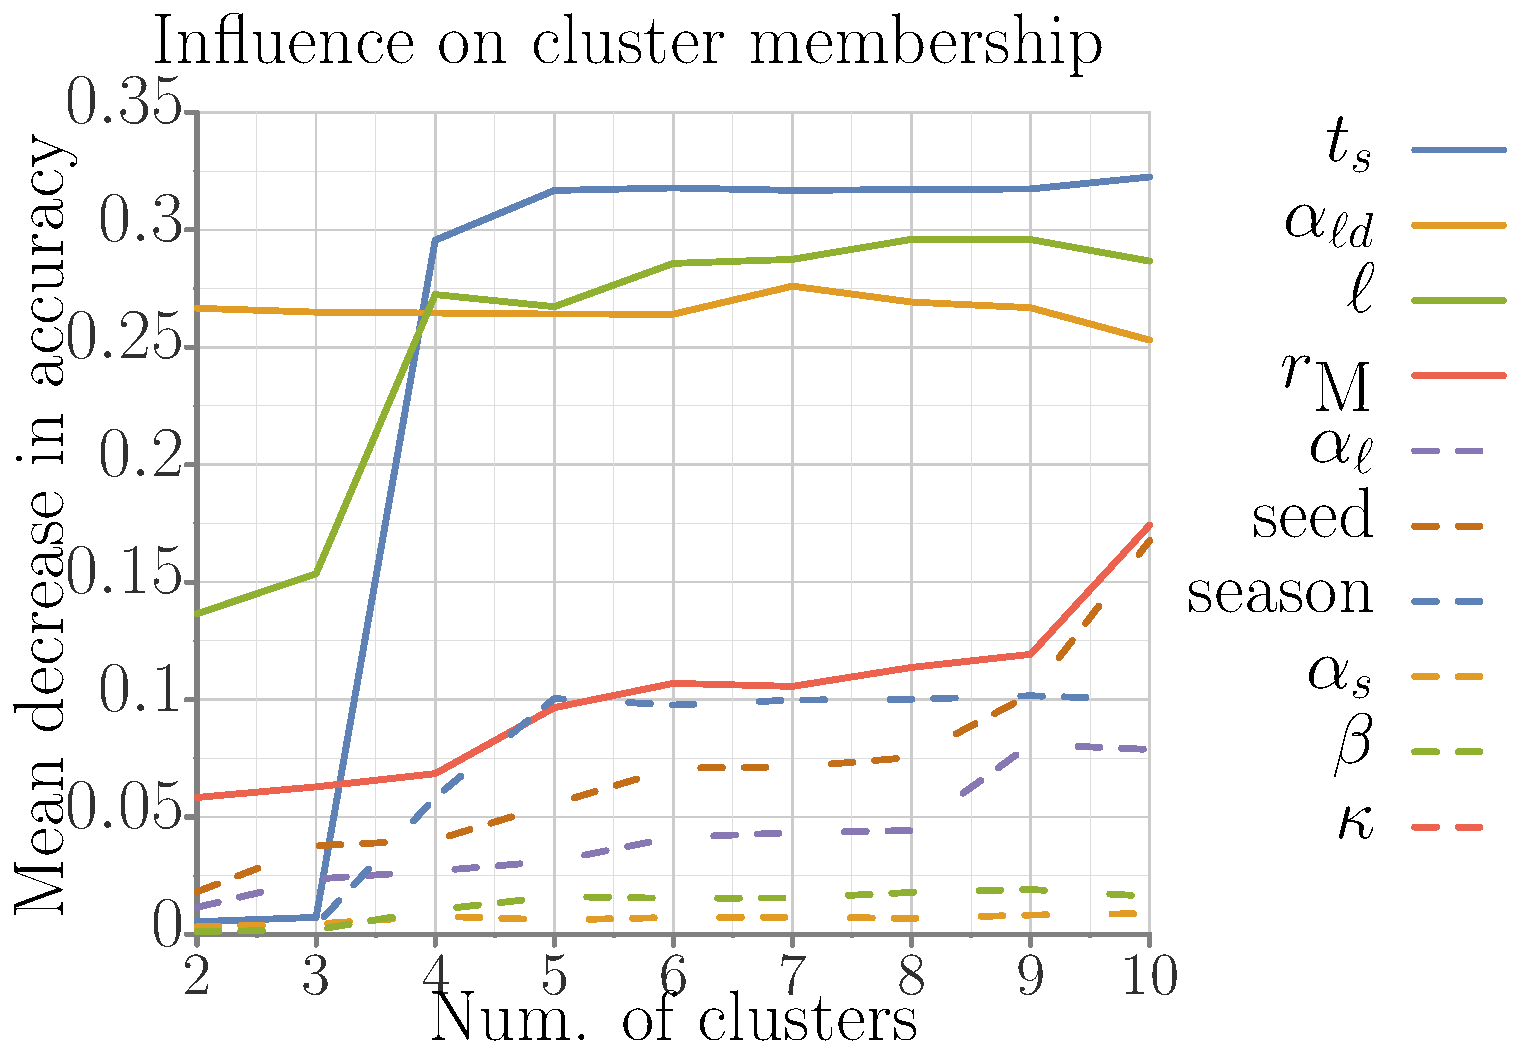
\includegraphics[width=0.9\textwidth]{../clustering/results/agglomerative/rf_k_agglomerative_mse.pdf}
    \caption{Parameter importance \label{fig:rf}}
\end{subfigure}
\caption{\textbf{Possible spread patterns in Bangladesh.} The contour plots
show the spread starting from the location of first report in Panchagarh
district for a simulation time of 12 months.  Here, the time of infection
for a cell is the minimum time step~$t$ such that the empirical probability
that the cell is infected by time~$t$ is $\ge0.8$. Also highlighted are the
eight monitored locations and the localities applied in the model. The
colours of the monitored locations correspond to the time of infection
relative to the first report (Panchagarh). Two distinct spread patterns
emerged from the cluster analysis. (a) and (b) show representative spreads
observed for each class. The similarity in each case was $\similarity>.8$.
Importance of model parameters with respect to (i)~similarity
score~$\similarity$ and (ii)~cluster membership based on random forest
method. The latter plot shows how the results vary with an increase in the
number of clusters for hierarchical clustering algorithm. More results are
presented in Figure~\ref{S:fig:rf} in the supplement. Videos depicting the
spatiotemporal spread for each class are provided of the supplement.
}
\end{figure}
%%

The Class~A spread pattern does not capture the gap between the time of first
report (Panchagarh) and the report in Gaibandha district
(Figure~\ref{fig:bgdClassA}). Even though the distance between the two
locations is only $185$km, the latter reported the presence only after~10
months of first report, suggesting that self-mediated spread might have been
much slower. In the model output on the other hand, the corresponding cell
gets infected between the second and fourth months.  In Class~B, this
location is infected much later in comparison. However, the eastward spread
towards the location Jaintiapur is slower than what was observed
(Figure~\ref{fig:bgdClassB1}). Even though Panchagarh is quite far from
this location, pest presence was reported by February 2017, just nine
months after the first report.  As a baseline, we also simulated the spread
using the cellular automata model developed by
Guimapi~\cite{guimapi2016modeling} for Bangladesh. The spread pattern is
similar to Class~A as the model does not account for long-distance hops.
However, the predicted rate of range expansion is much higher than our
models (see Section~\ref{S:sec:guimapi} for model details and results).

The relative importance of model parameters was assessed using random
forest algorithm with regard to their influence on (i)~similarity score
($\similarity$) and (ii)~spread pattern, which in our
case, is akin to cluster membership. In the case of spread pattern, the
importance was derived for each~$k$ (number of clusters) and clustering
algorithm. Some results are presented in Figure~\ref{fig:rf}. We note that
the long-distance scaling factor ($\ald$) is among the top three important
parameters. The start month ($t_s$) is also important for two reasons.
Firstly, the distance between two time shifted simulation outputs can be
large. Secondly, outputs are sensitive to seasonal variations or
temporality of the network.  Latency period ($\ell$) and Moore range
($\mooreRange$) together control the extent of radial spread in a time
step. Typically for Class~A models, $\mooreRange$ is high and $\ell$ is
low and the other way round in the case of Class~B models. Analysis of
trade flows and seasonality is presented in
Section~\ref{S:sec:locality_flows}
in the supplement.

\paragraph{Scenarios of pest introduction to countries in Southeast Asia.}
To identify routes of introduction to other countries in the region, we
applied both Class~A and Class~B models. The starting point of the spread
corresponds to the Panchagarh district (Figure~\ref{fig:bgdClassA}). Both model
classes strongly indicate that \tuta{} is already present in parts of
Myanmar (curves corresponding to time step 24, or two years from first
report). Also, the pest is likely to enter Thailand from Myanmar, and
subsequently move to Laos, Cambodia, and Vietnam as it spreads eastwards, and
to China when it spreads northwards. From Thailand, spreading southward, it
will enter Malaysia and subsequently enter Indonesia
(Figure~\ref{fig:msaClassAB}).


We also analysed the international tomato trade network
(Section~\ref{S:sec:tomnet} of supplement) to assess the risk due to
imports from \tuta{} infested countries outside this region.  Malaysia and
Singapore are important hubs with tomato imports from \tuta{} infested
regions. There is a possibility that \tuta{} is directly introduced to
these regions.  However, in both cases, the import volume is very low.
Also, the introduction risk depends on the preventive measures taken by the
exporting countries. With respect to both trade and natural pathways, there
is a low chance that the pest will be introduced into Philippines from
neighbouring countries, as there are no shared borders with any country in
the region nor evidence of tomato trade. However, human mobility is a
possible pathway. For example, the Middle East is the top destination for
Filipino workers.%%~\cite{rodriguez2011philippine}.
%%
\paragraph{Predicted spread is model and region dependent.} In the case of
Class~A models, the eastward spread is faster than southward spread
(Figure~\ref{S:fig:msaClassA} in the supplement). This is mainly because
the Moore neighbourhood is smaller at the narrow region in the south of
Myanmar and Thailand bordering Malaysia.  However, in the case of Class~B
(Figure~\ref{S:fig:msaClassB}), the spread is much faster in the same
region aided by domestic trade flows from northern and central Thailand to
the southern region. The Class~A spread pattern predicts that within the
next 4-5 years, much of the northern part of Mainland Southeast Asia will
be invaded.  The Class~B spread pattern predicts that in the same period,
\tuta{} will spread all over Malaysia and Singapore.  However, the rate of
spread observed is slower than that observed in Bangladesh for both
classes. Also, even though the models exhibited a similar rate of spread
for Bangladesh, we observed high variance in intensity of infestation as
well as range expansion for the rest of the region. The results are in
Figure~\ref{S:fig:spreadRate}. The reason for slow spread is as follows.
Bangladesh has the highest tomato volume per country surface area
($\approx2.5$tonnes/km$^2$).  The next country is Vietnam
($\approx1.5$tonnes/km$^2$). Therefore, in the case of Bangladesh, not only
is the extent of infestation in a cell~$\infest(\cdot)$ typically high, but
also since it is a densely populated country, most cells have vegetable
production. Hence, the rate of spread is much higher for relatively lower
values of pathway parameters and Moore range. Also, we observed a strong
dependence on Moore range (Figure~\ref{S:fig:spreadRateB}).  In
geographically larger countries, the production is scattered. Therefore,
the lower the Moore range, the slower the spread.

\paragraph{Influence of domestic trade on spread pattern and rate.}
Here, we focus on long-distance dispersal and therefore restrict our
discussion to Class~B models. For the country-specific studies, the
starting location was decided based on our analysis of possible entry
points through different pathways (Section~\ref{S:sec:seeds} in the
supplement).  We observed the following common spread pattern.  When the
invasive species is introduced to a country, dispersal is slow until the
invasion front reaches a {production source}. Once it establishes at a
source, the spread is very fast.  Depending on the country, within~12 to~24
time steps (or 1-2 years), it spreads to almost all major localities of
the country (see Figure~\ref{fig:thlBContourInt} for example). Production
areas which are very close to high-consumption localities (large urban
areas) are particularly vulnerable. Since local production typically does
not satisfy demands of such localities, they have high inflows from other
production areas and possibly from other countries. As a result, these
localities are quickly infected. Once introduced to such localities,
farmer--market interactions (local human-mediated dispersal) can facilitate
the introduction of the pest to nearby production regions where it can
establish and proliferate.

%%
Given that monitoring and quarantining are both resource intensive and
potentially disruptive, developing strategies that involve few locations
yet provide near-optimal control is a goal for modellers.  Market-level
phytosanitary measures in terms of import restrictions have been undertaken
by countries~\cite{USDA2012}. Here, we evaluated a simple strategy for
containing the spread through the trade pathway. Localities associated with
high annual outflows were identified (at most four in each country). As
discussed earlier, pest establishment in these areas can potentially lead
to rapid range expansion. The outflow from the targeted localities was cut
off to mimic control at the trade/market level. In the strictest sense,
this can be implemented by restricting trade of host crops. But, it is
possible that phytosanitary measures have the same effect.
Figure~\ref{fig:spread} shows results for two countries.  More results are
present in Figure~\ref{S:fig:intervene} in the supplement.  Consistently,
across countries, we observed a significant reduction in range expansion as
well as intensity of spread.  Besides, as seen in
Figure~\ref{fig:thlBContourInt}, stifling these flows localises the spread
that resembles those of Class~A models, but with much less intensity.
%%
\begin{figure}[pt]
\begin{subfigure}[b]{.28\textwidth}
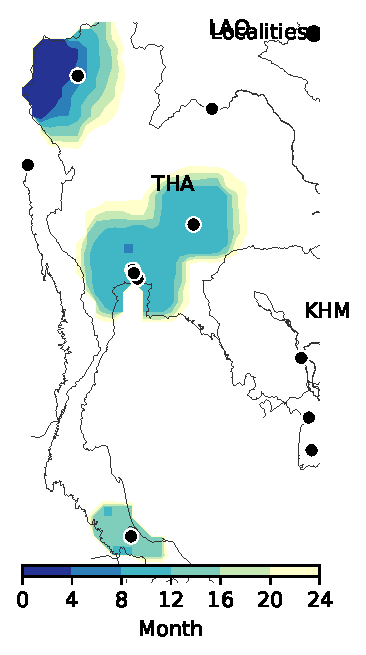
\includegraphics[width=\textwidth]{../cellular_automata/results/contour/TH_model-B_precip1_m1_l3.pdf}
\caption{Thailand without intervention\label{fig:thlBContour}}
\end{subfigure}
\begin{subfigure}[b]{.28\textwidth}
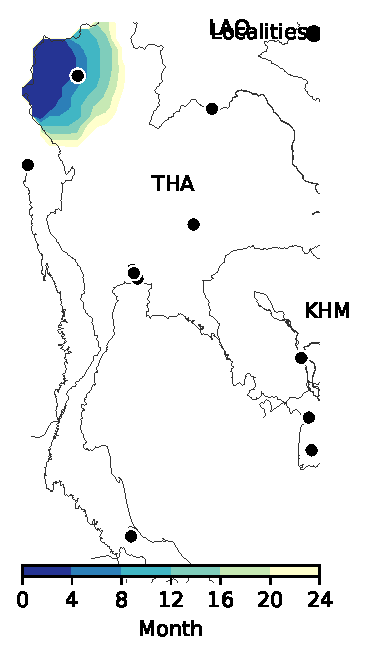
\includegraphics[width=\textwidth]{../cellular_automata/results/contour/TH_model-B_precip1-out-100_m1_l3.pdf}
\caption{Thailand with intervention\label{fig:thlBContourInt}}
\end{subfigure}
\begin{subfigure}[b]{.43\textwidth}
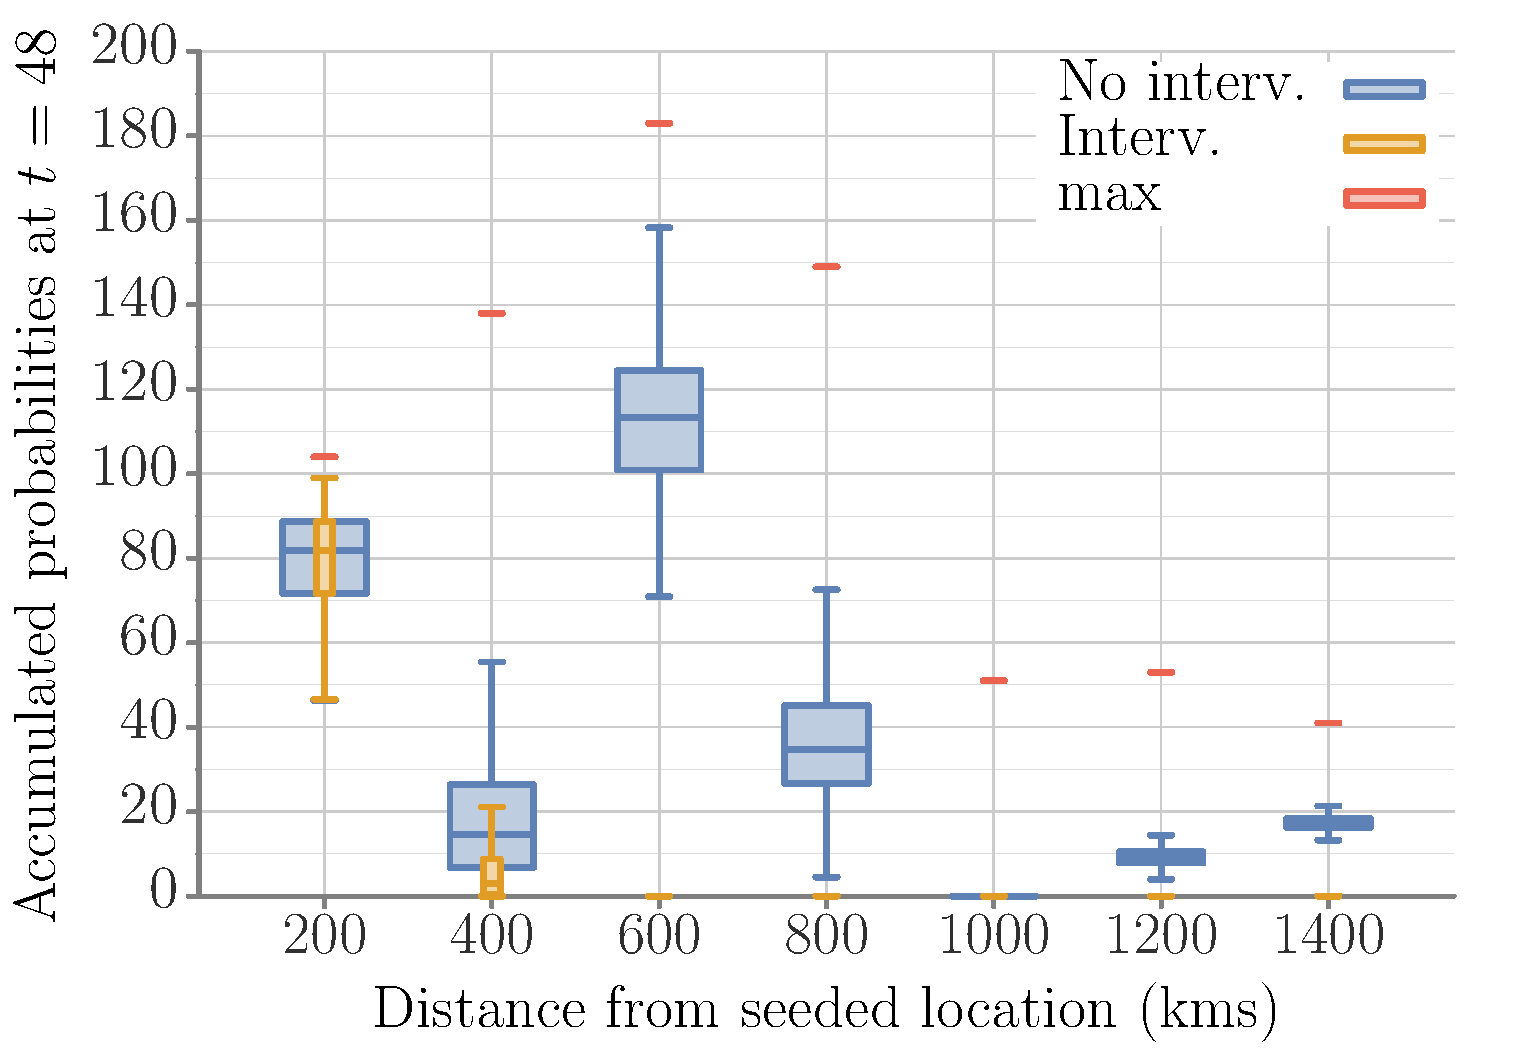
\includegraphics[width=\textwidth]{../cellular_automata/results/dist_inf_plots/TH_dist_prob_B_box.pdf}
\caption{Thailand: range of expansion (all Class B models)\label{fig:thlBContourBox}}
\end{subfigure}
%% \begin{subfigure}[b]{.28\textwidth}
%% 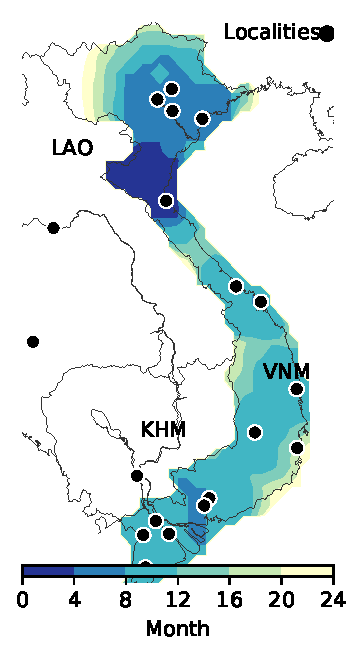
\includegraphics[width=\textwidth]{../cellular_automata/results/contour/VN_model-B_precip1_m1_l3.pdf}
%% \caption{Vietnam: without intervention\label{fig:vnmBContour}}
%% \end{subfigure}
%% \begin{subfigure}[b]{.28\textwidth}
%% 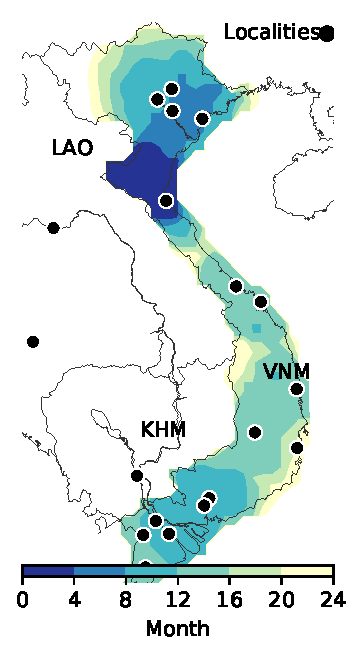
\includegraphics[width=\textwidth]{../cellular_automata/results/contour/VN_model-B_precip1-out-100_m1_l3.pdf}
%% \caption{Vietnam: with intervention\label{fig:vnmBContourInt}}
%% \end{subfigure}
%% \begin{subfigure}[b]{.43\textwidth}
%% 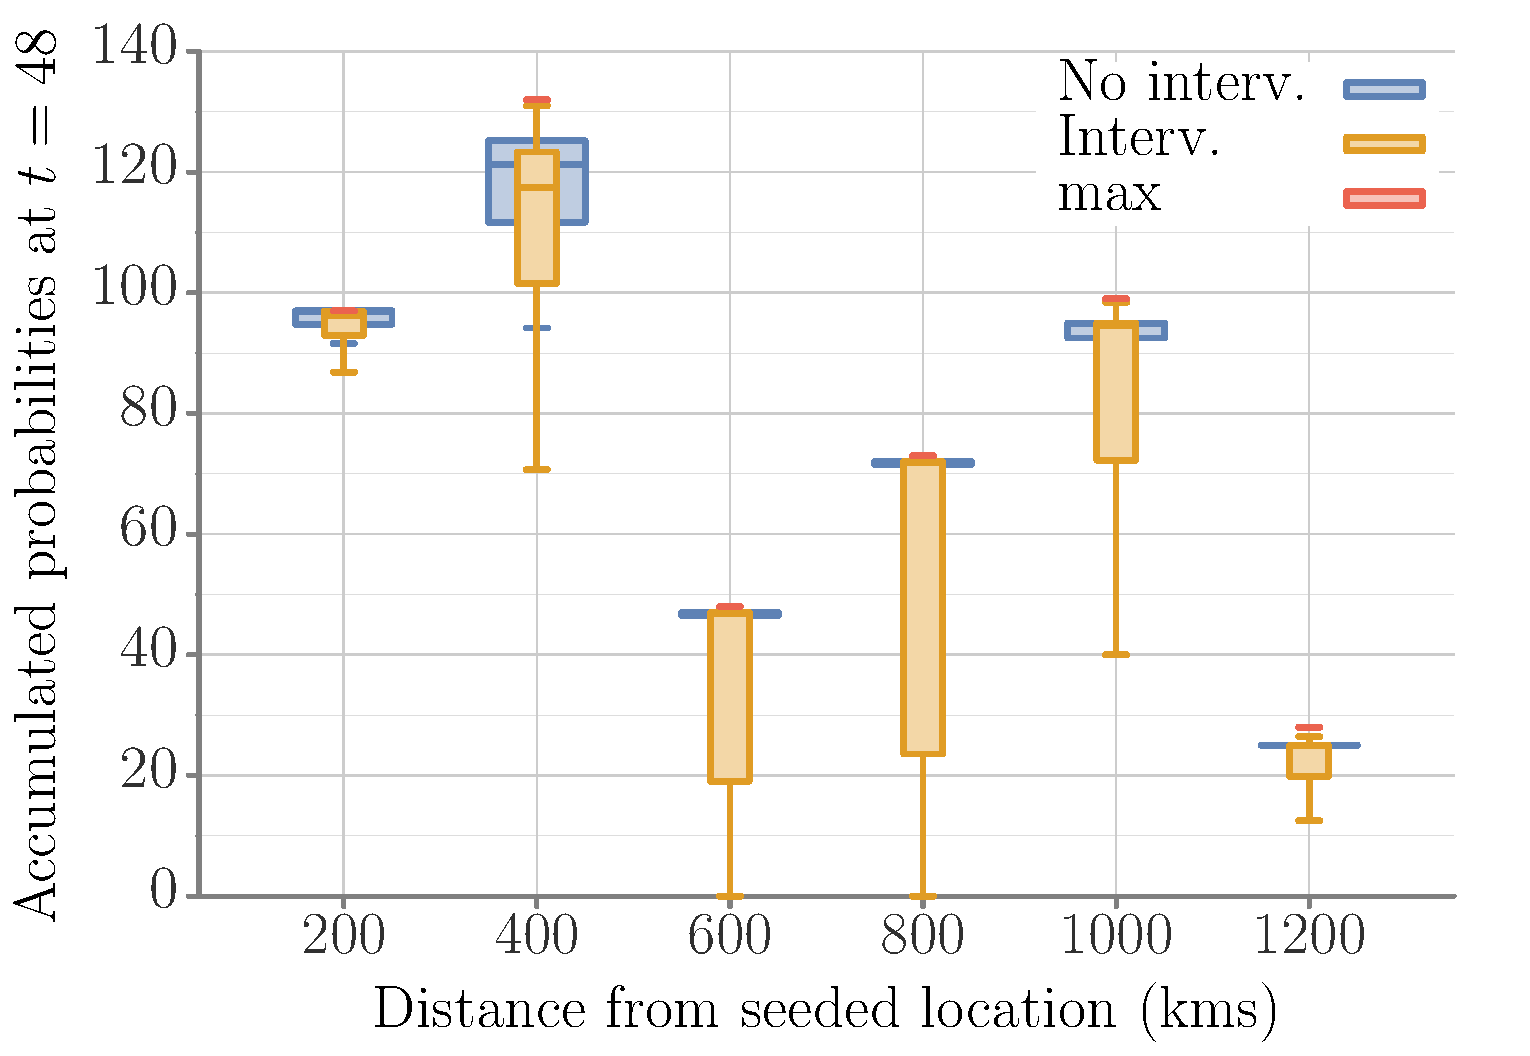
\includegraphics[width=\textwidth]{../cellular_automata/results/dist_inf_plots/VN_dist_prob_B_box.pdf}
%% \caption{Vietnam: range of expansion (all Class B models)\label{fig:vnmBContourBox}}
%% \end{subfigure}
\caption{\textbf{Rate and pattern of spread with and without intervention.}
Representative spread dynamics of Class~B models ($\mooreRange=1, \ell=3$)
for two countries. More plots are shown in Figure~\ref{S:fig:intervene}. In each
case, a cell close to a high production region was seeded. The first column
corresponds to spread for 48 months after introduction. The colours indicate
the time interval at which there is at least a 50\% chance that a location
will be infected.The second column corresponds to spread after cutting off
flows from chosen localities. The third column shows average spread with
respect to origin of infection for all Class~B models. The cells are binned
based on their distance from the origin of infection. Given time step~$t$
(48), let $\Pr_{\le t}(v)$ be the probability that cell~$v$ is in state~$I$
by time~$t$. For each configuration, we computed the ``total
infection'' for every bin at time~$t$ by aggregating~$\Pr_{\le t}(v)$ for
each~$v$ in the bin. The red points referred to as ``max'' correspond to
the total number of cells in each bin, which is also the maximum possible
accumulated probability for that bin.
\label{fig:spread}}
\end{figure}

%%
\section{Discussion}
The variability in the spread patterns that explain the incidence reports
exposes the lack of understanding of the pathways of spread.  Nevertheless,
the analysis does strongly indicate the role of human-assisted spread of
\tuta{}. The pest was reported in May~2016 in the northwestern part of
Bangladesh bordering India. The region is among the top three tomato
producers in the country. By the beginning of the next production season,
\tuta{} was found in almost every major urban region.  Similar correlation
between tomato trade and \tuta{} spread was observed in
Nepal~\cite{venkatramanan2019modeling}. Studies on self-mediated spread
(flying capability or by wind) can definitely help estimate more accurately
the rate of self-mediated spread. It is also important to consider
alternate scenarios of introduction. We recall that the far eastern part of
Bangladesh (locality Jaintiapur in Figure~\ref{fig:bgdClassB1}) reported
pest presence nine months after the first report. In a typical Class~B
spread pattern, however, this region was not infected within that time
frame mainly because of weak trade flows to that region. However, in
January 2017, \tuta{} was officially reported from Meghalaya in India,
about 100km from Jaintiapur. It also happens to be near an important trade
route from India to Northeastern Bangladesh. Therefore, it is possible that
multiple incursions took place. It is possible that analysis of other
countries or regions can reduce this variability. But caution needs to be
exercised before applying analysis of one region to another, as trade
dynamics, and production methods. Thus, pathways can vary widely from
one region to another.

Historically, international trade has played a strong role in the spread of
\tuta{} between countries. For example, the pest was first reported by
India in~2014. By early~2016, it was discovered in the Kathmandu area of
Nepal and in the northern part of Bangladesh in May~2016. Both countries import
significant volumes of tomatoes from India. However, there has been no report
from Pakistan, another neighbour which does not import tomato from India.
There are similar examples outside the region such as its slow advance from
South America to Central America, or the fact that it is not reported in
China despite being present in neighbouring Central Asian countries
since~2015.  We recall the discussion on slow predicted rate of spread in
Mainland Southeast Asia compared to the observed rate in Bangladesh. One
reason for this could be the unaccounted trade flows between countries.
International trade within this region is not documented well.  It is
critical to address the data gaps concerning international trade,
particularly considering that production and trade between countries in
this region have been increasing over the years (details are in
Section~\ref{S:sec:tomnet} of supplement).

While several integrated pest management strategies have been suggested
for managing \tuta{}, hardly any work has been done in designing effective
interventions at the trade level. Designing phytosanitary measures targeted
towards markets and vehicles of transportation for preventing introductions
(or reintroductions) is therefore a promising research direction. Some
countries have already taken measures in this regard. Our results also
indicate that monitoring markets with inflows from many regions is
important. In the United States for example, the Animal and Plant Health
Inspection Service of the Department of Agriculture (USDA-APHIS) has
instituted quarantine regulations for imports from regions where the pest
is present~\cite{USDA2012}. Identifying the optimal set of nodes in a
network to reduce infectious disease spread is a widely studied topic.
There are very few works that apply such techniques to invasive species
spread~(Nopsa~et~al.~\cite{nopsa2015ecological} for example). As the world
moves towards concentrated and specialised agricultural production,
focusing on this aspect becomes increasingly important.
%%~\cite{madar2004immunization}
%%
\paragraph{Literature survey.} Multi-pathway models are being increasingly
used to study the role of invasive species dispersal.
Douma~et~al.~\cite{douma2016pathway} survey the literature categorising
various efforts into flow-based pathway models and agent-based models.
Carrasco~et~al.~\cite{carrasco2010unveiling} combine spatially
explicit models of human-mediated spread with a phenology model to
incorporate population dynamics of the western corn rootworm.
Nopsa~et~al.~\cite{nopsa2015ecological} use a network science approach to
study the role of transport and storage infrastructure in the spread of
pests and pathogens of wheat. Our model is in part motivated by the hybrid
approaches used in the study of infectious diseases of humans and
livestock~\cite{bradhurst2015hybrid,yang2016}.
Although there is a general consensus that vegetable and seedling trade is
a primary driver of \tuta{} spread, previous modelling efforts have
exclusively focused on ecological aspects. Several
studies~\cite{desneux2010biological,tonnang2015identification} provide risk
maps using CLIMEX and take additional factors into account.
Guimapi~et~al.~\cite{guimapi2016modeling} used a cellular automata approach
to capture the global spread of the pest by factoring in temporal
variations and spatial distribution of vegetation, temperature, and tomato
production. A precursor to this work~\cite{venkatramanan2019modeling}
modelled the seasonal production and trade of tomato in Nepal to study the
role of trade in the spread of \tuta{} using a gravity model and
network dynamics.

Emulators --based on Gaussian processes for
example~\cite{fadikar2018calibrating} -- and machine learning
surrogates~\cite{lamperti2018agent} are emerging as solutions to overcome
computational challenges, parameterization, and sensitivity analysis of
complex agent-based models. The parameter importance study and
parameterization was partly motivated by the work of
Lamperti~et~al.~\cite{lamperti2018agent}. We are not aware of any previous
work that analyses the dynamics of simulation systems using unsupervised
learning as presented in this paper. However, clustering has been considered
in the context of multi-resolution simulation models as an interfacing
component between simulators with different
resolutions~\cite{cassandras2000clustering}. We cast the problem of
deriving relationship between model parameters and cluster index as a
classification problem. CART was our choice of algorithm since the
learned model is a decision tree that can be interpreted. In principle, any
such algorithm which provides such an explanation (such as multinomial
regression for example) can be employed.

%%
\paragraph{Challenges and limitations.} Modelling emerging invasions is
particularly challenging. Limited data on incidence and understanding of
the underlying dynamics makes it nearly impossible to calibrate and
validate the models.   We have had to simplify or ignore some of the
processes that might significantly influence the spread.  For example, our
model uses monthly production as a surrogate for infectiousness of a cell.
Complex phenology models can be used instead (as in
Carrasco~et~al.~\cite{carrasco2010unveiling}), but would add to the
complexity of the model.
Since our focus region spans multiple countries, identifying and collecting
data for each country was a lengthy process. For many countries, data had
to be collected (or even inferred) from several publications and reports
(Table~\ref{S:tab:countryData}). Further, these datasets were misaligned in
time and spatial resolution.  It is important to account for heterogeneity
in production, consumption, awareness, cultural factors, etc. both within
and between countries.  Some countries are technologically more advanced
than others, which manifests as differences in yield, crop loss, trade
infrastructure, pest awareness, and preparation for
invasion~\cite{early2016global}.

In particular, it is hard to model human-assisted spread owing to lack of
seasonal trade data. To determine outflows and inflows for each locality,
we had to identify major ports for import(s) and export(s) as well as
estimate the fraction of production which was used for processing and was
available only for a few countries. The farm--market-consumer interactions
(local human-mediated spread) involves various actors such as farmers,
wholesalers, retailers, wet markets, supermarkets, and so on. Modelling
this is a challenge in itself. If data on actual flows of vegetables is
provided, the gravity model can be improved or replaced by more
sophisticated approaches. Also, the relationship between long-distance
invasion risk and trade volume is hard to determine. While a direct
relationship between volume and risk is plausible, whether the relation is
linear (as assumed by our model) is unclear.

\paragraph{Conclusion.} Traditionally, in developing countries, crops such
as tomato are seasonal. However, over the past decade, due to rising demand and
opportunities to export, there has been a thrust towards year-round
production using protected cultivation methods and resilient varieties.
An increase in urban population, short shelf life of vegetables, and the
advantages of short marketing chains have encouraged urban agriculture in
developing countries~\cite{moustier2015urban}. Our results indicate that
such urban and peri-urban agriculture is particularly vulnerable to
invasive species attacks. In particular, in Southeast Asia, vegetable
production and internal trade have steadily increased. In comparison, the
export of tomato outside of the focus region has risen steeply in 
recent years (after 2011), while the imports generally indicate a downward
trend.  Therefore, invasions from pests such as \tuta{} can have a huge
negative impact on the socioeconomic fabric of this region. The modelling
and analysis framework presented here is generic and applicable to other
invasive species.  The methodology is modular and leverages popular
learning algorithms to analyse complex models under data scarcity.  Other
potential applications for this work include studies of natural or
human-initiated disasters, climate change, and optimisation of food flows.
\paragraph{Data availability.} The authors declare that the data supporting the
findings of this study are available within the paper and its Supplementary
Information file, or from the authors upon reasonable request.

\paragraph{Acknowledgements}
This work was supported in part by the United States Agency for
International Development under the Cooperative Agreement NO.
AID-OAA-L-15-00001 Feed the Future Innovation Lab for Integrated Pest
Management, DTRA CNIMS Contract HDTRA1-11-D-0016-0001, NSF BIG DATA Grant
IIS-1633028, NSF DIBBS Grant ACI-1443054, NIH Grant 1R01GM109718 and NSF
NRT-DESE Grant DGE-154362.  We are grateful to Yousuf Mian, Nguyen Van Hoa,
and Kimhian Seng for their help with obtaining country-specific information
on production, trade, and pest incidence. We thank Richard Beckman, Irene
Eckstrand and Erin Raymond for useful discussions on model design and paper
organisation.

\paragraph{Author contributions.}
AA defined the scope of the
research. AA, JM, TB, MRC collected and interpreted data.
AA, MM conceived and designed the
experiments. JM, AA and YYC performed the
analysis. HM, ND, TB and RM provided assistance in interpreting the
results. AA and JM wrote the paper with significant inputs from
MRC and YYC. AA supervised the research. All authors discussed the
results and commented on the manuscript.

\bibliographystyle{abbrv}
\bibliography{refs}
%%
\end{document}
